\documentclass [11pt, a4paper]{article}

\usepackage[left=1.5cm, text={18cm, 25cm}, top = 2.5cm]{geometry}
\usepackage{times}
\usepackage{amsmath}
\usepackage{amsthm}
\usepackage{amsfonts}
\usepackage[czech]{babel}
\usepackage[utf8]{inputenc}
\usepackage[IL2]{fontenc}
\usepackage{verbatim}
\usepackage{graphics}
\usepackage{graphicx}
\usepackage[unicode]{hyperref}
\usepackage{enumitem}
\usepackage{float}

\begin{document}
\begin{center}

%%% Title page %%%
\Huge
\textsc{Fakulta informačních technologií\\
Vysoké učení technické v Brně}
\\[84mm]
\Huge \textbf{Dokumentácia -- IFJ 2018}\\
\LARGE Tím 40, varianta II
\vspace{\stretch{9.5}}
\end{center}


\hfill

%%% Names %%%
\begin{minipage}[l]{0.6 \textwidth}
\Large
\begin{tabular}{l l l}
Adam Hostin  & xhosti02  & \quad25\,\%\\
Sabína Gregušová & xgregu02 & \quad25\,\% \\
\textbf{Dominik Peza}  & \textbf{xpezad00}  & \quad\textbf{25\,\%}\\
Adrián Tulušák  & xtulus00  & \quad25\,\%\\
\end{tabular}
\end{minipage}




\thispagestyle{empty}
\clearpage

%%% Content table %%%
\setcounter{page}{1}
\tableofcontents
\clearpage


\section{Úvod}
Naším cieľom je implementovať prekladač imperatívneho jazyka IFJ18 do predmetov IFJ a IAL v jazyku C. Hlavnou náplňou práce bola implementácia: lexikálneho analyzátora, parsera (syntaktická a sématická analýza) a generátora inštrukcií.

\section{Lexikálna analýza}
Na začiatku sme implementovali lexikálny analyzátor v súbore \texttt{lexer.c}, ktorého základom je deterministický konečný automat (ďalej iba DKA).  Hlavnou funkciou v tomto súbore je \texttt{get\_next\_token}, ktorá číta jednotlivé znaky a pomocou príkazu \texttt{switch} prechádza do nasledujúcich stavov podľa DKA až kým nevyhodnotí  lexikálne správny token, inak vracia \texttt{ER\_LEX}. Lexikálny analyzátor musí mať nadstavený vstupný súbor, ktorý obsahuje program napísaný v jazyku IFJ18.

Pri úspešnom vyhodnotení tokenu sa správne uvoľní všetká alokovaná pamäť. Matematické a relačné operátory sú vyhodnotené vcelku rýchlo a jednoducho, identifikátory, reťazce a čísla vyžadujú viacej prechodov a používajú dynamický reťazec, o ktorom ďalej pojednáva sekcia Spracovanie reťazcov. Pri identifikátore sa kontrolujú povolené znaky na základe pozície v reťazci a na záver sa identifikátor porovná so všetkými kľúčovými slovami, ak sa nájde zhoda, je to kľúčové slovo, inak je to identifikátor. Reťazce sú ohraničené dvojitými úvodzovkami (") a môžu obsahovať escape sequence. Pre tento prípad existuje špeciálny stav \texttt{STATE\_BACKSLASH\_LITERAL}, do ktorého sa prechádza pri  prečítaní znaku \textbackslash \quad a čaká sa na skratku escape sequence, ako napríklad t, s alebo n. 

\subsection{Štruktúra Token\_t}
Pre jednoduchšiu prácu s tokenmi sme použili štruktúru \texttt{Token\_t}, ktorá obsahovala:

\begin{itemize}
\item \textbf{union Token\_attr}
\item \textbf{struct Token\_type}
\end{itemize}
\textbf{Union Token\_attr} obsahuje možné atribúty tokenu, konkrétne to sú: string, integer, flt a keyword. \\
\textbf{Struct Token\_type} obsahuje typy tokenov, konkrétne to sú: \texttt{EOF}, \texttt{EOL}, identifikátor, kľúčové slovo, relačné a matematické operátory, ľava a pravá zátvorka, čiarka, komentár, int, float a string.


\subsection{Spracovanie reťazcov}
Pre jednoduchšie spracovanie reťazcov sme sa rozhodli implementovať súbor \texttt{dynamic\_string.c}. Jeho súčasťou je aj štruktúra \texttt{string\_t}, ktorá obsahuje samotný ukazateľ na dynamický reťazec, súčastnú veľkosť reťazca a celkovú veľkosť bufferu. Na začiatku je alokovaný reťazec s veľkosťou 10 bytov a pri každom pridaní znaku sa kontroluje, či je ešte v reťazci miesto. Keď sa blížime k zaplneniu reťazca, funkcia \texttt{check\_empty\_bites} zväčší veľkosť buffera o 5, čím zaistí dostatočnú veľkosť pre reťazec. Všetky alokácie pamäte sú kontrolované a ich zlyhanie je adekvátne ošetrené vrátením internej chyby \texttt{ER\_INTERNAL}.

\section{Syntaktická analýza}

\subsection{Precedenčná analýza výrazov}
Syntaktická analýza výrazov je implementovaná v súbore \texttt{expression.c} pomocou precedenčnej tabuľky. Hlavné telo \texttt{expression.c} pozostáva z funkcie \texttt{handle\_expression}, ktorá postupne spracováva jednotlivé tokeny alebo symboly a vyhodnocuje ich syntaktickú správnosť. Keďže nie je vždy úplne jednoznačne možné určiť, či nasledujúci token bude súšasťou výrazu alebo nie, rozhodli sme sa implementovať jednosmerne viazaný zoznam s pracovným názvom \texttt{buffer}, kam sa postupne ukladajú tokeny vždy na koniec zoznamu.

 Ak parser vyhodnotí, že dané tokeny nie sú súšasťou výrazu, vyčistí buffer a a syntaktická analýza pokračuje v parseri. V opačnom prípade je zavolaná funkcia \texttt{handle\_expression}, ktorá pri spracovaní používa tokeny v bufferi, až kým nie je buffer prázdny a ďalej si žiada tokeny pomocou funkcie \texttt{get\_next\_token}. Z každého tokenu si vytvoríme symbol na základe jeho typu, ktorý si ďalej ukladáme na zásobník. Spracovávanie symbolov je naprogramované na základe algoritmu uvedeného v prezentácii \cite{IFJpred}. Symboly majú svoj status, ktorý sa kopíruje aj pri redukcii danej časti výrazu. Časti výrazu sa postupne dávajú na zásobník generátora a akonáhle už raz bol daný výraz daný do generátora, jeho status sa mení na \texttt{ON\_GENERATOR\_STACK} a pri daľšej redukcii už nebude znova pridaný na zásobník generátora. 

Pri spracovaní výrazov máme flag \texttt{return\_code}, ktorý môže nadobúdať hodnotu:
\begin{itemize}
\item \textbf{EXPRESSION\_OK} - výraz má správnu syntax aj sématiku
\item \textbf{SYNTACTICAL\_ERRORS} - výraz má syntaktickú chybu
\item \textbf{UNDEFINED\_ID\_EXPRESSION} - výraz má sématickú chybu
\item \textbf{ER\_INTERNAL} - interná chyba (neúspešný malloc, neúspešné pridanie do zásobníku a pod.)
\end{itemize}

Pri kontrole jednotlivých symbolov na zásobníku sa zároveň kontroluje aj tento flag, a jeho nadstavenie na čokoľvek iné ako \texttt{EXPRESSION\_OK} vedie na ukončenie spracovávania výrazov s adekvátnym návratovým kódom.

\subsection{Sématická analýza}
Sématickú analýzu sme implementovali ako tabuľku s rozptýlenými položkami. Synonymá sú v tabuľke zoradené explicitne, čo zabezpečuje tereticky neobmedzený počet položiek uchovávateľných tabuľkou symbolov. Synonymá sú zreťazené v jednosmerne viazaných zoznamoch. Veľkosť mapovacieho poľa sme vyberali tak, aby bola rovná prvočíslu. Naša tabuľka má veľkosť 6421. Očakávame, že naplnenie tabuľky nepresiahne 75\%. Mapovaciu funkciu sme prevzali z druhej domácej úlohy z IAL, lebo nám pripadala efektívna a ľahko pochopiteľná. 

Funkcia spočítava ASCII hodnotu jednotlivých znakov kľúča a nakoniec vracia modulo veľkosti tabuľky z daného súčtu. Každá položka tabuľky obsahuje svoj vlastný unikátny kľúč, ktorý sa ukladá v podobe reťazca. Kľúče značia identifikátory funkcii a premenných. Každá položka taktiež obsahuje svoj typ, značiaci či sa jedná o premennú alebo funkciu, boolovskú hodnotu, určujúca či bola položka definovaná, ukazateľ na ďalší prvok v zozname a integer značiaci počet parametrov v prípade, že sa jedná o funkciu. Položky sa ukladajú do 2 identických tabuliek s rozptýlenými položkami v závislosti od toho, či sa jedná o lokálne alebo globálne premenné. Všetky funkcie sa ukladajú do globálnej tabuľky symbolov. Implementovali sme taktiež niekoľko funkcii zabezpečujúce pohodlnú prácu s tabuľkou. Funkcie zabezpečujú inicializáciu, výpis chybových hlásení, pridávanie prvkov, vyhľadávanie v tabuľke, kontrolu jednotlivých atribútov položiek a čistenie tabuľky.

\section{Generovanie inštrukcií}

\section{Práca v tíme}
<<<<<<< HEAD
Náš tím sme si zostavili pomerne skoro. Po rozdelení práce na menšie celky sme začali každý pracovať na časti pridelenej vedúcim tímu. Približne 3 týždne pred pokusným odovzdaním sme začali jednotlivé časti spájať do celku. Pokusné odovzdávanie sme využili, no výsledok nás nemilo prekvapil. Zistili sme, že hoci všetko fungovvalo pomerne správne, návratové hodnoty sme vždy "natvrdo" vracali buď ako 0 alebo 1, čo sa aj prejavilo na celkovom percentuálnom hodnotení. Pri tejto príležitosti sme spravili riadnu revíziu kódu a poopravovali čo najviac chýb a nedostatkov. Práca v tíme bola rozdelená nasledovne:

\begin{table}[H]
\centering
\begin{tabular}{|l|l|}
\hline
Meno & Povinnosti\\ \hline
\textbf{Dominik Peza} & vedenie tímu, pridelovanie úloh, kontrola práce, konzultácie, generovanie inštrukcií\\
Sabína Gregušová & lexikálna analýza, precedenčná analýza výrazov, dokumentácia, testovanie\\
Adam Hostin & sématická analýza, tabuľka symbolov, dokumentácia, testovanie, diagramy\\
Adrián Tulušák & syntaktická analýza, sématická analýza, testovanie, dokumentácia\\
\hline
\end{tabular}
\end{table}
=======
Náš tím sme si zostavili pomerne skoro. Po rozdelení práce na menšie celky sme začali každý pracovať na časti pridelenej vedúcim tímu. Približne 3 týždne pred pokusným odovzdaním sme začali jednotlivé časti spájať do celku. Pokusné odovzdávanie sme využili, no výsledok nás nemilo prekvapil. Zistili sme, že hoci všetko fungovvalo pomerne správne, návratové hodnoty sme vždy "natvrdo" vracali buď ako 0 alebo 1, čo sa aj prejavilo na celkovom percentuálnom hodnotení. Pri tejto príležitosti sme spravili riadnu revíziu kódu a poopravovali čo najviac chýb a nedostatkov. 
>>>>>>> parent of 4c8da57... Updated makefile

\subsection{Komunikácia}
Už na začiatku sme sa dohodli na pravidelných týždenných stretnutiach, kde sme diskutovali o našej ďaľšej práci na nadchádzajúci týždeň. Komunikovali sme najmä cez facebook a skype a osobné stretnutia boli veľmi príjemné. 

\subsection{Verzovanie}
Pre správu projektu sme používali verzovací systém Git a vzdialený repozitár GitHub. Tento spôsob správy projektu nám umožňoval pracovať na viacerých častiach projektu súčasne. Po otestovaní jednotlivých podčastí sme súbory začali spájať do celku a každý mal možnosť testovať projekt už ako celok.

\subsection{Hodnotenie}
Celkovo hodnotíme tento projekt kladne, hoci na začiatku vyzeral pomerne zložito, postupne sme mali nápady ako dané problémy vyriešiť a nakoniec sme všetko stihli v časovom predstihu, takže sme mali možnosť odstraňovať chyby a testovať správnosť a určite tento projekt prispel k zlepšeniu našich programátorských schopností.
\newpage
\bibliographystyle{czechiso}
\renewcommand{\refname}{Použitá literatúra}
\bibliography{doc}

\newpage
\appendix

\section{Deterministický konečný automat}
<<<<<<< HEAD
\scalebox{0.85}{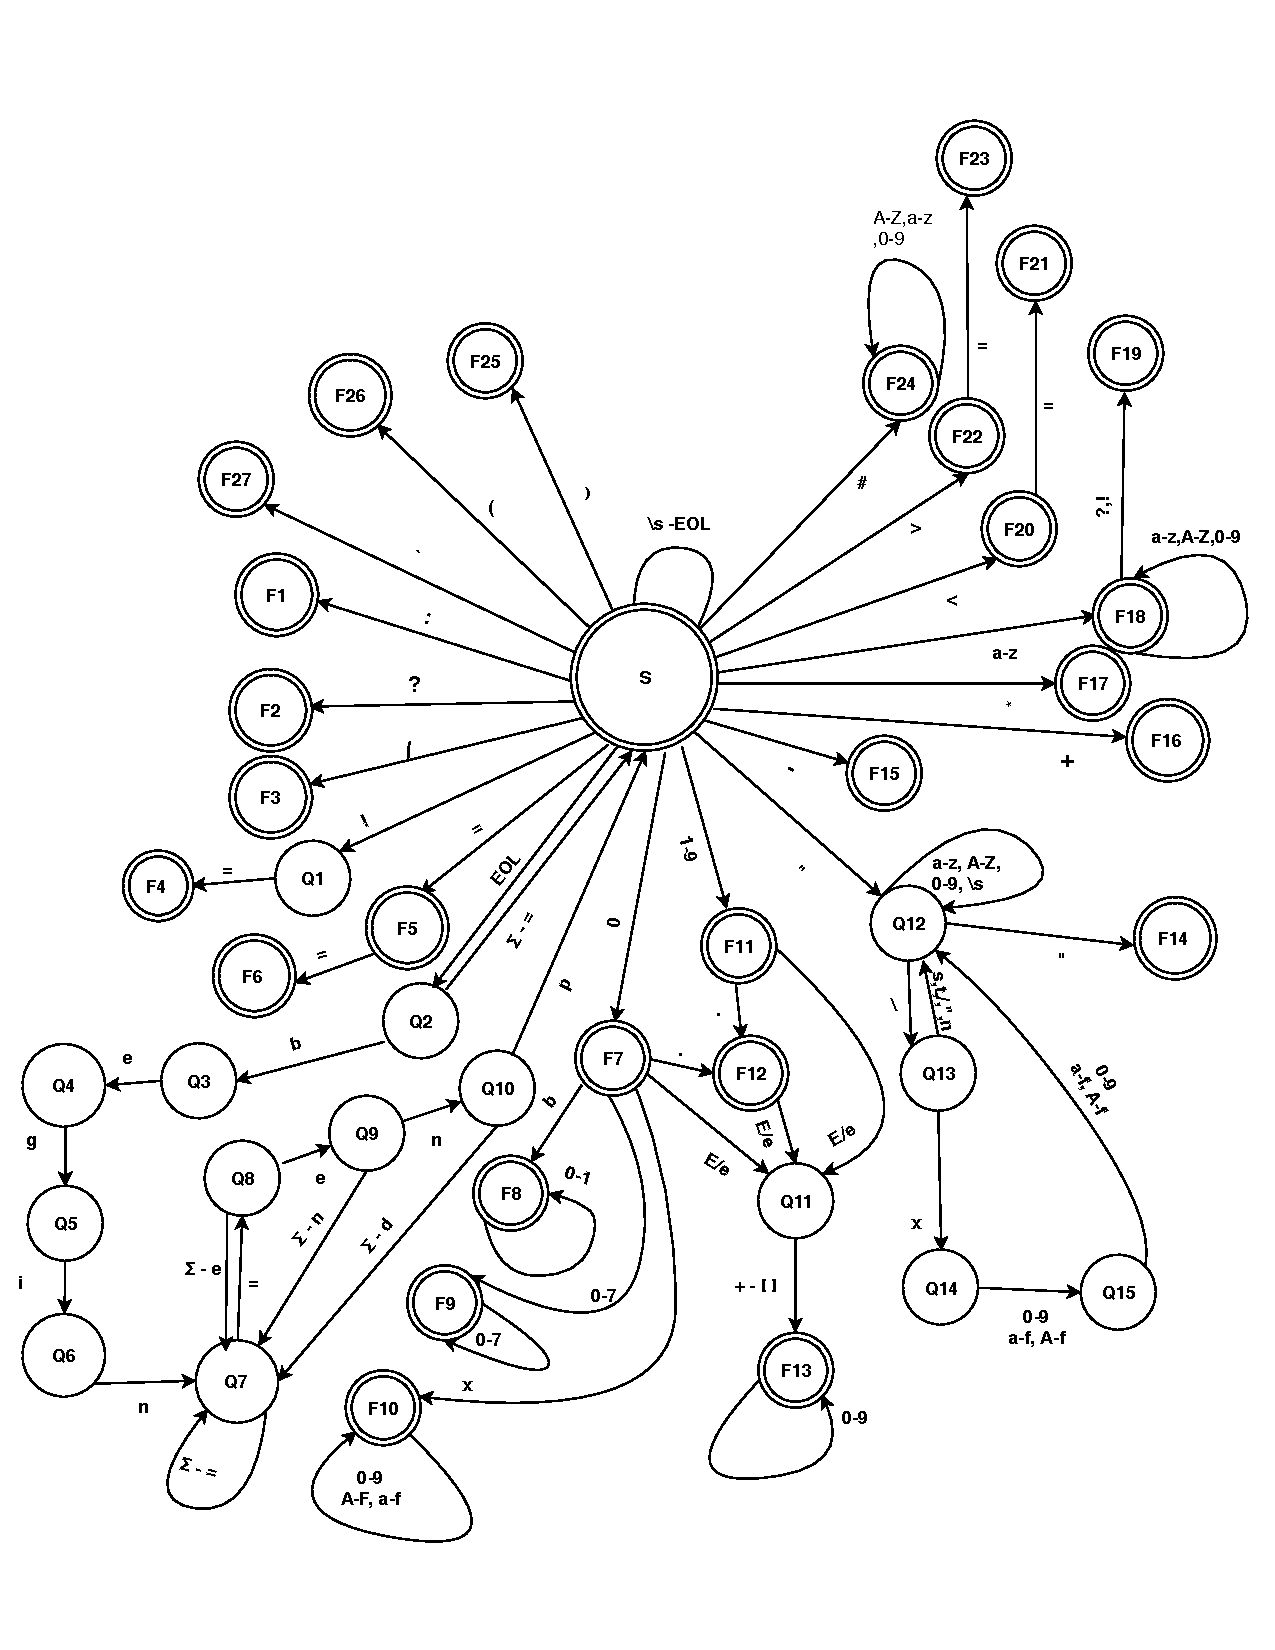
\includegraphics{DKA.pdf}}

=======
>>>>>>> parent of 4c8da57... Updated makefile
\section{LL-gramatika}
\begin{table}[!ht]
	\centering
    \begin{enumerate}[noitemsep]
        \item \verb|<prog> -> DEF ID_FUNC ( <params> ) EOL <statement> END <prog>|
        \item \verb|<prog> -> EOL <prog>|
        \item \verb|<prog> -> EOF|
        \item \verb|<prog> -> <statement> <prog>|
        
        \item \verb|<statement> -> IF <expression> THEN EOL <statement> ELSE| \\ 
\verb|EOL <statement> END <prog>|
        \item \verb|<statement> -> WHILE <expression> DO EOL <statement> END EOL|
        \item \verb|<statement> -> <function> EOL|
        \item \verb|<statement> -> ID EOL|
        \item \verb|<statement> -> ID <declare> EOL|
        \item \verb|<statement> -> EOL <prog>|
        
        \item \verb|<declare> -> = <value>|
        \item \verb|<declare> -> = <expression>|
        \item \verb|<declare> -> = <function>|
        \item \verb|<declare> -> |$\varepsilon$
        
        \item \verb|<params> -> ID <param>|
        \item \verb|<params> ->| $\varepsilon$
        
        \item \verb|<param> , ID <param>|
        \item \verb|<param> -> |$\varepsilon$
    
        \item \verb|<argvs> -> <value> <arg>|
        \item \verb|<argvs> -> |$\varepsilon$
        
        \item \verb|<arg> -> , <value> <arg>|
        \item \verb|<arg> ->| $\varepsilon$
        
        \item \verb|<value> -> INT_VALUE|
        \item \verb|<value> -> FLOAT_VALUE|
        \item \verb|<value> -> STRING_VALUE|
        \item \verb|<value> -> ID|
       
        \item \verb|<function> -> PRINT ( <argvs> ) EOL|
        \item \verb|<function> -> LENGTH ( <argvs> ) EOL|
        \item \verb|<function> -> SUBSTR ( <argvs> ) EOL|
        \item \verb|<function> -> ORD ( <argvs> ) EOL|
        \item \verb|<function> -> CHR ( <argvs> ) EOL|
        \item \verb|<function> -> INPUTS EOL|
        \item \verb|<function> -> INPUTI EOL|
        \item \verb|<function> -> INPUTF EOL|
        \item \verb|<function> -> ID_FUNC ( <argvs> )|
	\end{enumerate}

	\label{table:ll_gramatika}
\end{table}
\section{Precedenčná tabuľka}
\begin{table}[H]
\centering
\begin{tabular}{|c|c|c|c|c|c|c|c|c|c|}
\hline
   & \textbf{+} & \textbf{\--}  & \textbf{*} & \textbf{/} & \textbf{(} & \textbf{)} & \textbf{i}  & \textbf{R} & \textbf{\$} \\ \hline
\textbf{+}  & \textgreater{} & \textless{}    & \textless{}    & \textless{}    & \textless{} & \textgreater{} & \textless{} & \textgreater{} & \textgreater{} \\ \hline
\textbf{\--}  & \textgreater{} & \textgreater{} & \textless{}    & \textless{}    & \textless{} & \textgreater{} & \textless{} & \textgreater{} & \textgreater{} \\ \hline
\textbf{*}  & \textgreater{} & \textgreater{} & \textgreater{} & \textgreater{} & \textless{} & \textgreater{} & \textless{} & \textgreater{} & \textgreater{} \\ \hline
\textbf{/}  & \textless{}    & \textgreater{} & \textgreater{} & \textgreater{} & \textless{} & \textgreater{} & \textless{} & \textgreater{} & \textgreater{} \\ \hline
\textbf{(}  & \textless{}    & \textless{}    & \textless{}    & \textless{}    & \textless{} & =              & \textless{} & \textless{}    &                \\ \hline
\textbf{)}  & \textgreater{} & \textgreater{} & \textgreater{} & \textgreater{} &             & \textgreater{} &             & \textgreater{} & \textgreater{} \\ \hline
\textbf{i}  & \textgreater{} & \textgreater{} & \textgreater{} & \textgreater{} &             & \textgreater{} &             & \textgreater{} & \textgreater{} \\ \hline
\textbf{R}  & \textless{}    & \textless{}    & \textless{}    & \textless{}    & \textless{} & \textgreater{} & \textless{} &                & \textgreater{} \\ \hline
\textbf{\$} & \textless{}    & \textless{}    & \textless{}    & \textless{}    & \textless{} &                & \textless{} & \textless{}    &                \\ \hline
\end{tabular}
\end{table}



\end{document}
